
\section{Introduction}

Reinforcement learning (RL) is an area of research that focuses on finding an action that will maximize a reward function given the state of an agent. Finding the optimal action requires large amounts of data gathered from the agent interacting with the environment. The ability to gather reliable data is crucial to the learning process because this provides the learning algorithm with an accurate representation of how the state evolves with a given action. 

RL has recently become a topic of interest due to its ability to solve problems with dynamics that can be difficult, if not impossible, to model given computational limitations. The underlying problem of complex dynamics can be addressed using model-free reinforcement learning and is widely used over a large set of applications including control theory, natural language processing, image recognition, and medical diagnoses. The most common model-free reinforcement learning algorithm is call Q-learning and it relies on applying incremental estimation to the Bellman equation.

\begin{equation}
	Q(s,a) \leftarrow Q(s,a)+\alpha(r + \gamma \max_{a'} Q(s',a') - Q(s,a))
\end{equation}

Model-free learning can be applied online (updating the Q values after each action) or applied as an offline strategy using batch learning (gathering data for a fixed period of time and updating the Q values). Online implementations require the runtime of the update equation to not interfere with the agents ability to perform an action at the next available time step. Batch learning is a simple yet effective method to apply reinforcement learning to an agent in a time critical scenario that may not be able to update its knowledge between each action taken.

Super Smash Bros Melee presents an environment with dynamics that are difficult to model without knowledge of the underlying engine used to build the game. In addition to complex dynamics, the game has a state space that would be infeasible to represent as discrete values. A model-free approach eliminates the need for a state transition model and generalization allows the agent to approximate the optimal policy given limit data. Given the nature of the problem we would like to solve, we chose to implement a perceptron Q-learning algorithm. In this algorithm, a set of weights for each action $\theta_a$ is trained on a basis function $\beta(s)$, such that the state-action value can be globally approximated as $Q(s,a) = \theta^T_a\beta(s)$. The weights are trained in batches after each game is complete. This was done to ensure that the agent is able to select an optimal action at each time step and is not waiting for weight updates.

\begin{equation}
	\theta_a \leftarrow \theta_a+\alpha(r + \gamma \max_{a'} \theta_{a'}^T\beta(s',a') -  \theta_{a}^T\beta(s,a))\beta(s,a)
\end{equation}

Super Smash Brothers Melee is a platform based fighting game in which the goal is to knock your opponent off of the stage. Damage dealt to the opponent increases the distance they fly when hit. At its core, the strategy can be distilled into dealing damage to the opponent and knocking them off when possible while simultaneously avoiding your opponents attempts to do the same. While the game has many available characters and stages, we limited the project to a single stage (Final Destination) and character (Captain Falcon) for convenience of training, although the work done should allow for training of any character and stage.

\begin{figure}[!htb]
\centering
	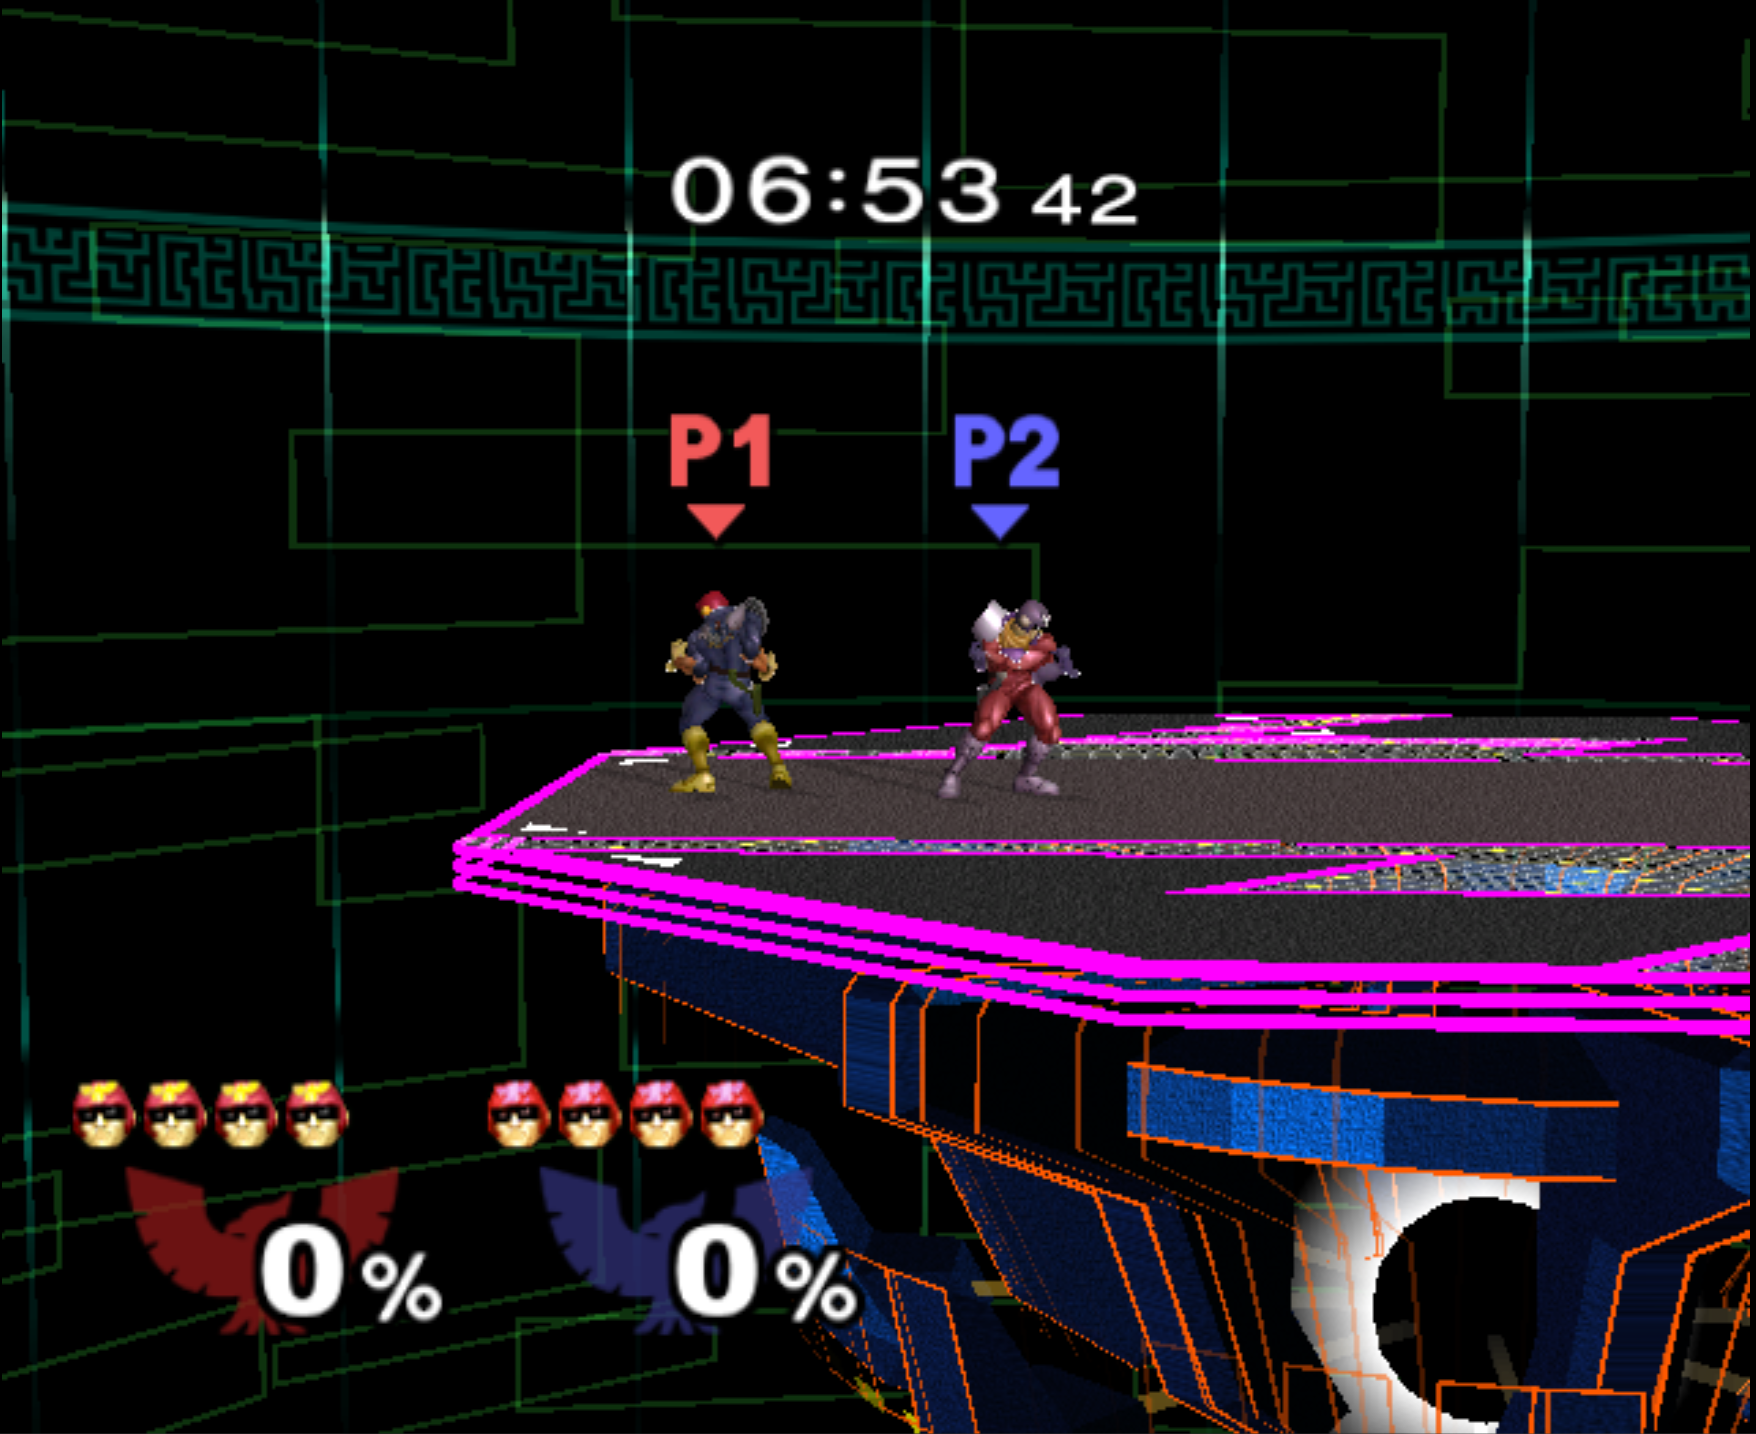
\includegraphics[width=80mm]{stage.png}
	\caption{Screenshot of Super Smash Brothers Melee environment. \label{melee}}
\end{figure}

To interact with the game environment, we leveraged the open-source game emulator Dolphin as well as the python library libmelee which provides a python interface for reading state values and issuing controller inputs. We define the action space as $\mathbb{A}$ and the state space as $\mathbb{S}$. The action space contains a set of actions that are mapped to a combination of buttons being pressed on a gamecube controller. The state space contains a set of continuous and discrete variables that represent the agent and its opponent in the environment.





